\subsubsubsubsection{Standard scheduler}
\begin{figure}[h]
\centering
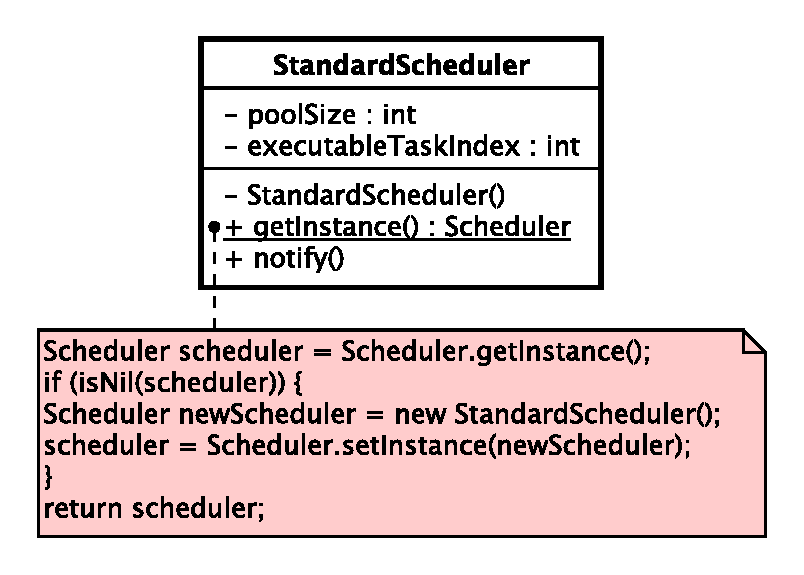
\includegraphics[scale=0.6,keepaspectratio]{images/solution/app/backend/standard_scheduler.eps}
\caption{\pScheduling::StandardScheduler}
\label{fig:sd-app-scheduling-standard-scheduler}
\end{figure}
\FloatBarrier
\begin{itemize}
  \item \textbf{\descr} \\
    A concrete Scheduler implemeting Scheduler abstract methods in a traditional way.
    Ensures the existence of at most one instance of the class, 
 	and provides a global point of access to it.
  	Uses lazy initialization, hence no class instance is created 
  	or stored until one is first requested.
    It is a singleton because only one traveller scheduler is needed.
  \item \textbf{\ops}
  \begin{itemize}
    \item \texttt{StandardScheduler()} \\
    Private and unique constructor because the class has the exclusive 
    responsability for instancing it.
    \item[+] \texttt{\underline{getInstance() : District}} \\
    Static method lets clients access the unique instance 
    of \texttt{Scheduler}. At the first invocation, it is responsible 
    for creating the instance.
    \item[+] \texttt{notify()} \\
	Notifies of changes all the attached Traveller objects.
  \end{itemize}
\end{itemize}
